% !TeX program = lualatex
% !TeX encoding = utf8
% !TeX spellcheck = uk_UA

\documentclass{LabWork}
\graphicspath{{LabWork6pic/}}
%============================================= Заголовок документу ====================================================%
\work{6}
\title{Магнітний момент у магнітному полі}

%\author{Тор А.~В.}{}
%\author{Другий А.~В.}{}
%
%\group{ФФ-93}

\abstract{Визначити момент сили, зумовлений магнітним моментом в постійному магнітному полі, як функцію:
\begin{itemize}
\item індукції магнітного поля;
\item кута між напрямком магнітного поля та магнітного моменту;
\item величини магнітного моменту.
\end{itemize}
За результатами експериментів визначити константу котушок Гельмгольца.
}
%======================================================================================================================%

\begin{document}
\writedatatofile{\jobname}
\maketitle


\section{Теоретичне підґрунтя}
\subsection{Що таке магнітний момент}

\textbf{Магнітний момент}, або \textbf{магнітний дипольний момент} --- векторна величина, що характеризує взаємодію тіла з магнітним полем.

Означення магнітного моменту:
\begin{equation}\label{eq:definition}
	\tcbhighmath[drop fuzzy shadow]{
		\vec{p}_m = \frac12 \int\limits_V \vec{r} \times \vec{j} dV,
	}
\end{equation}
де $\vec{j} dV$~--- елемент об'ємного струму. У випадку елемента лінійного струму $I\vec{dl}$ формула~\eqref{eq:definition} перетворюється на вираз:
\begin{equation}\label{eq:definition_linear_element}
	\tcbhighmath[drop fuzzy shadow]{
		\vec{p}_m = \frac{I}{2} \oint\limits_L \vec{r} \times \vec{dl}.
	}
\end{equation}
Використовуючи формулу~\eqref{eq:definition_linear_element} можна знайти момент кільцевого витка зі струмом:

\begin{equation}\label{eq:circuit}
	\tcbhighmath[drop fuzzy shadow]{
		\vec{p}_m = IS\vec{n},
	}
\end{equation}
де $\vec{n}$~--- вектор нормалі до плоскої поверхні витка. Напрямок вектора нормалі співпадає з правилом правого гвинта (рис.~\ref{pic:gimlet}).

%---------------------------------------------------------
\begin{wrapfigure}{O}{0.5\linewidth}\centering
	\begin{tikzpicture}
		\node[anchor=south west,inner sep=0] at (0,0) {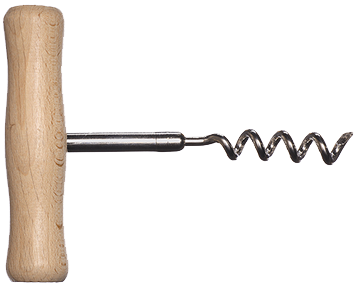
\includegraphics[]{corksckrew}};
		\draw [thick, red, decoration={
					markings,
					mark=at position 0.5 with {\arrow{latex}}}, postaction={decorate}](1.5,1.25) [ partial ellipse =5:355:0.25 and 1];
		\draw[blue, -latex, thick] (3, 1.25) -- (4, 1.25) node[below] {$\vec{n}$} node[right, black] {рух гвинта};
		\node[blue] at (2,2) {$N$};
		\node[red] at (1,2) {$S$};
	\end{tikzpicture}
	\caption{Полюса витка}
	\label{pic:gimlet}
\end{wrapfigure}
%---------------------------------------------------------

Магнітне поле впливає на магнітний диполь. Зокрема, на виток зі струмом, що вміщений в однорідне магнітне поле діє обертовий момент:
\begin{equation}\label{eq:Torque}
	\tcbhighmath[drop fuzzy shadow]{
		\vec{M} = \vec{p}_m\times \vec{B}.
	}
\end{equation}
Вираз~\eqref{eq:Torque} є фундаментальним фактом, тобто достовірність має бути перевірена на досліді.

Зокрема, вираз~\eqref{eq:Torque} дає можливість ввести кількісну характеристику  магнітного поля~--- \emph{вектора індукції}.

Для цього необхідно взяти виток з одиничним магнітним моментом, який ми визначили за формулою~\eqref{eq:circuit}. Для  того, щоб магнітний момент витка був одиничним, необхідно, щоб по ньому йшов струм в $I = 1$~Ампер, а площа такого витка дорівнювала $S = 1$~м$^2$. Розташуємо тепер виток так, щоб його магнітний момент був перпендикулярним до магнітного поля і виміряємо момент сили, тоді це значення і буде те число, яким ми кількісно охарактеризуємо магнітне поле\footnote{Характеристику магнітного поля --- індукцію --- не можна ввести аналогічно до того способу, яким вводиться характеристика електричного поля --- напруженість, тобто через силу, що діє на одиничний заряд, оскільки в природі не існує магнітного заряду (\href{https://en.wikipedia.org/wiki/Magnetic_monopole}{монополя}) }:
\begin{equation}\label{B}
	B = \frac{M}{p_m}.
\end{equation}
Ця величина назвається індукцією магнітного поля. В системі одиниць SI, ця величина вимірюється в Теслах, скорочено -- Tл:
\begin{equation}
	1 \text{Тл} = \frac{\text{1 Н}\cdot\text{м}}{\text{А}\cdot\text{м}^2}.
\end{equation}


\subsection{Котушки Гельмгольца}

Котушки Гельмгольца (кільця Гельмгольца) --- пристрій, що складається з двох однакових тонких соленоїдів, розташованих на одній осі на відстані один від одного, що дорівнює їх радіусам (рис.~\ref{pic:Helmholtz_coils}) і які з'єднані послідовно таким чином, щоб струм у них циркулював в однаковому напрямку. Котушка названа на честь \href{https://en.wikipedia.org/wiki/Hermann_von_Helmholtz}{Германа фон Гельмгольца}. Розташування двох соленоїдів на віддалі радіуса один від одного забезпечує таку однорідність поля вздовж осі, при якій відмінною від нуля є тільки четверта похідна від поля. Використовуються для отримання постійного, змінного або імпульсного магнітного поля з зоною однорідності, яке зазвичай використовується в експериментах, а також для калібрування датчиків магнітної індукції, намагнічування і розмагнічування постійних магнітів, розмагнічування сталевих заготівок, деталей і інструментів. Область поля з неоднорідністю менше $1$~\% є еліпсоїдом обертання близьким до сфери радіусом $0.3R$, що майже в $4$ рази більше ніж для одного кільця. Еліпсоїд трохи стислий уздовж осі (рис.~\ref{pic:Helmholtz_coils_field}).

%=========================================================
\begin{figure}[h!]\centering
	%---------------------------------------------------------
	\begin{minipage}[t]{0.45\linewidth}\centering
		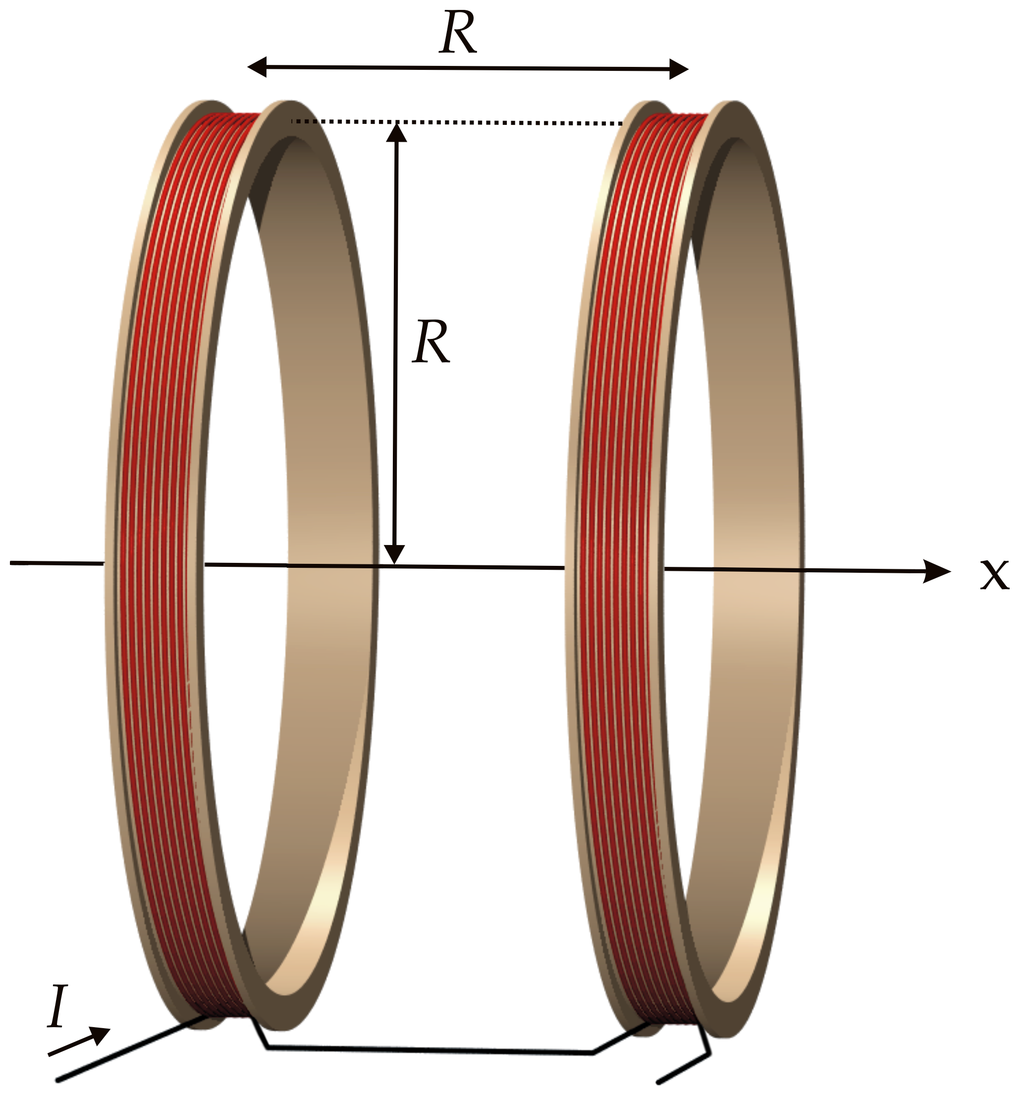
\includegraphics[width=0.8\linewidth]{Helmholtz_coils}
		\caption{Схема котушок Гельмгольца (взято з \href{https://en.wikipedia.org/wiki/Helmholtz_coil}{wikipedia})}
		\label{pic:Helmholtz_coils}
	\end{minipage}
	\qquad%---------------------------------------------------------
	\begin{minipage}[t]{0.45\linewidth}\centering
		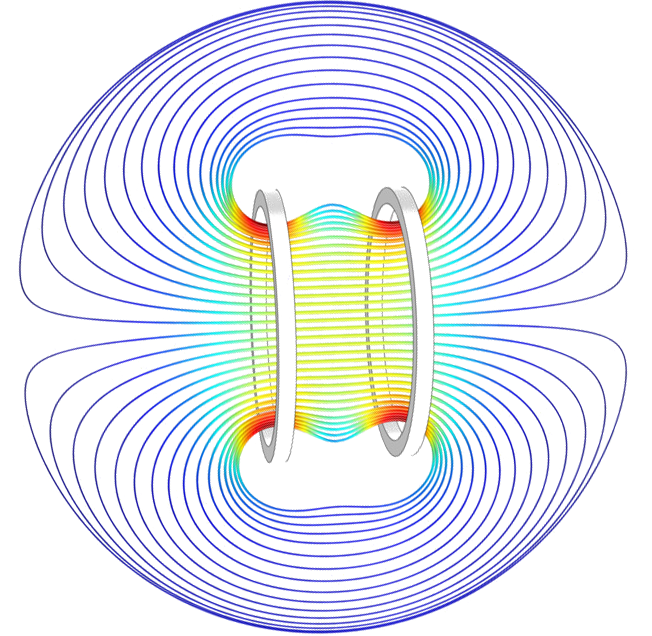
\includegraphics[width=0.8\linewidth]{Helmholtz_coils_field}
		\caption{Вигляд поля котушок Гельмгольца (взято з \href{https://www.freepng.ru/png-d02278/}{https://www.freepng.ru/png-d02278/})}
		\label{pic:Helmholtz_coils_field}
	\end{minipage}
	%---------------------------------------------------------
\end{figure}
%=========================================================

Магнітне поле в центрі між котушками можна розрахувати за допомогою закону Біо-Савара-Лапласа, який дає формулу:
\begin{equation}\label{eq:Helmholtz_coils_field}
		B = \left( \frac45\right)^{\frac32} \frac{\mu_0 nI}{R}.
\end{equation}
Константою котушок називається величина $C = \frac{B}{I}$, яка, як випливає з~\eqref{eq:Helmholtz_coils_field} визначається формулою:
\begin{equation}\label{eq:Helmholtz_coils_constant}
	\tcbhighmath[drop fuzzy shadow]{
		C = \left( \frac45\right)^{\frac32} \frac{\mu_0 n}{R},
	}
\end{equation}
де $n$~--- кількість витків в одному кільці, $R$~--- радіус кільця.

%
\fputrue% ----- Увімкнення двигуна точних розрахунків
\pgfmathsetmacro{\muz}{4*pi*1e-7}
\pgfmathsetmacro{\R}{0.2}
\pgfmathsetmacro{\n}{154}
\pgfmathsetmacro{\CG}{(4/5)^(3/2)*\muz*\n/\R}
\fpufalse% ----- Вимкнення двигуна точних розрахунків
%
\begin{wraptable}{O}{0.65\linewidth}\small
	\centering
	\caption{Параметри котушок}
	\begin{tabular}{ll}
		\toprule
		Величина                         & Значення                              \\ \midrule
		Кількість витків в одному кільці & $N = \pgfmathprintnumber[]{\n}$       \\
		Радіус кільця                    & $R = \pgfmathprintnumber[]{\R}$ м     \\ \midrule
		Константа котушок                & $C = \pgfmathprintnumber[]{\CG}$ Тл/А \\ \bottomrule
	\end{tabular}
	\label{tab:Helmgoltz_coils}
\end{wraptable}
В даній лабораторній роботі використовуються котушки Гельмгольца, параметри яких подані в  табл.~\ref{tab:Helmgoltz_coils}.


Розраховане значення константи котушок за формулою~\eqref{eq:Helmholtz_coils_constant} з використанням даних таблиці~\ref{tab:Helmgoltz_coils} дає значення:

\begin{equation}\label{val:Helmhottz_constant}
	C = \pgfmathprintnumber[sci, precision=2]{\CG}~\text{Тл/А}.
\end{equation}


\section{Робоча формула}

Якщо магнітне поле буде неоднорідним, то воно буде різне на різних частини  контура, який вміщений у це магнітне поле і, відповідно, на різні частини контура діяти різний обертальний момент.Для того, щоб цього уникнути, бажано використовувати однорідне магнітне поле, що забезпечується завдяки котушкам Гельмгольца.

У даній роботі контур~--- це пласка петля, що має $N$ витків, по якій тече постійний струм $I'$, діаметр кільця $d$. А тому, його магнітний момент дорівнює згідно з~\eqref{eq:circuit}:
\begin{equation*}\label{eq:pmE}
	p_m = I'\frac{N \pi d^2}{4},
\end{equation*}
а обертальний момент згідно~\eqref{eq:Torque} тоді визначатиметься як:
\begin{equation*}\label{}
	M = I'\frac{N \pi d^2}{4} B\sin\alpha.
\end{equation*}

Далі, враховуючи, що магнітне поле котушок Гельмгольца пропорційні силі струму, що тебе по ним ($B = CI$, де $C$~--- величина, що залежить від параметрів котушок і називається \emph{константою котушок Гельмгольца}) можемо записати:
\begin{equation}\label{eq:TorqueE}
	M = \frac{\pi}{4} CII'Nd^2\sin\alpha.
\end{equation}

\section{Експериментальне устаткування}

Експериментальне устаткування (рис.~\ref{pic:Experimental_installation}) складається з котушок Гельмгольца, крутильних терезів (моментометру) з пристроєм для утримання електричного контура, двох стабілізованих джерел живлення (рис.~\ref{pic:Power_supply}), двох амперметрів і набору контурів. Обладнання слід збирати так, як показано на схемі~рис.~\ref{pic:scheme_for_Helmholtz}. Зверніть увагу, що котушки Гельмгольца з'єднуються між собою послідовно. Дроти, що підводять струм до контуру мають звисати вільно і повинні бути скручені разом, щоб не створювати додатковий обертальний момент.
%=========================================================
\begin{figure}[h!]\centering
	%---------------------------------------------------------
	\begin{minipage}[t]{0.47\linewidth}
		\begin{tornpage}\centering
			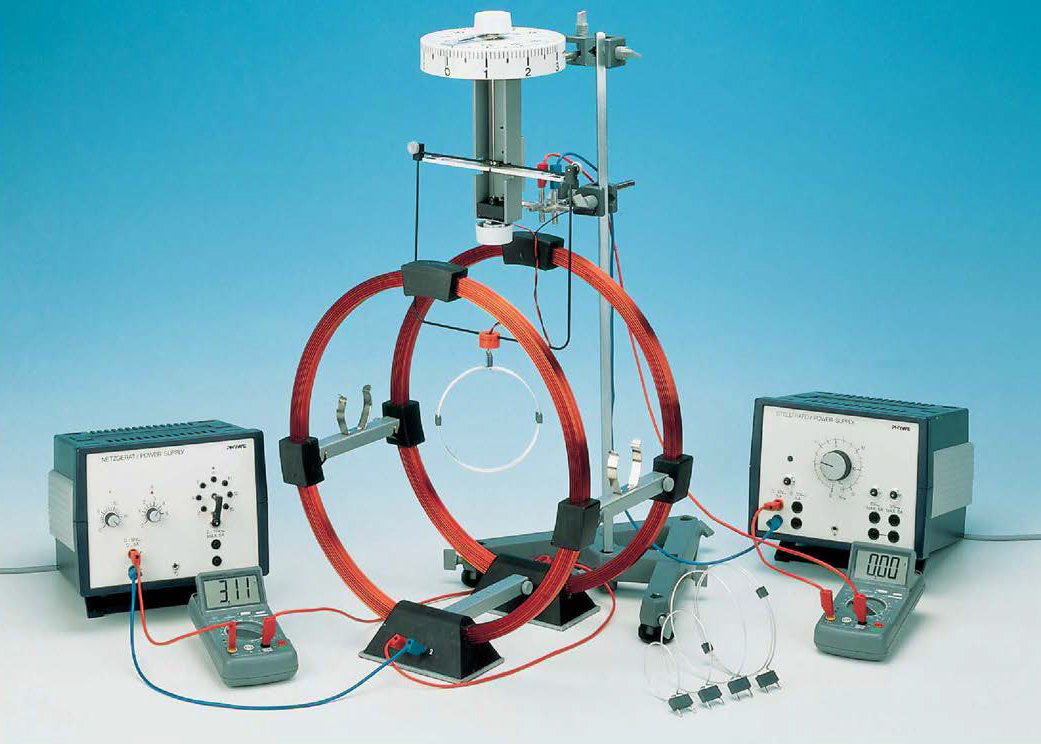
\includegraphics[width=1\linewidth]{Experimental_installation}
			\caption{Експериментальна установка}
			\label{pic:Experimental_installation}
		\end{tornpage}
	\end{minipage}
	\quad%---------------------------------------------------------
	\begin{minipage}[t]{0.47\linewidth}
		\begin{tornpage}\centering
			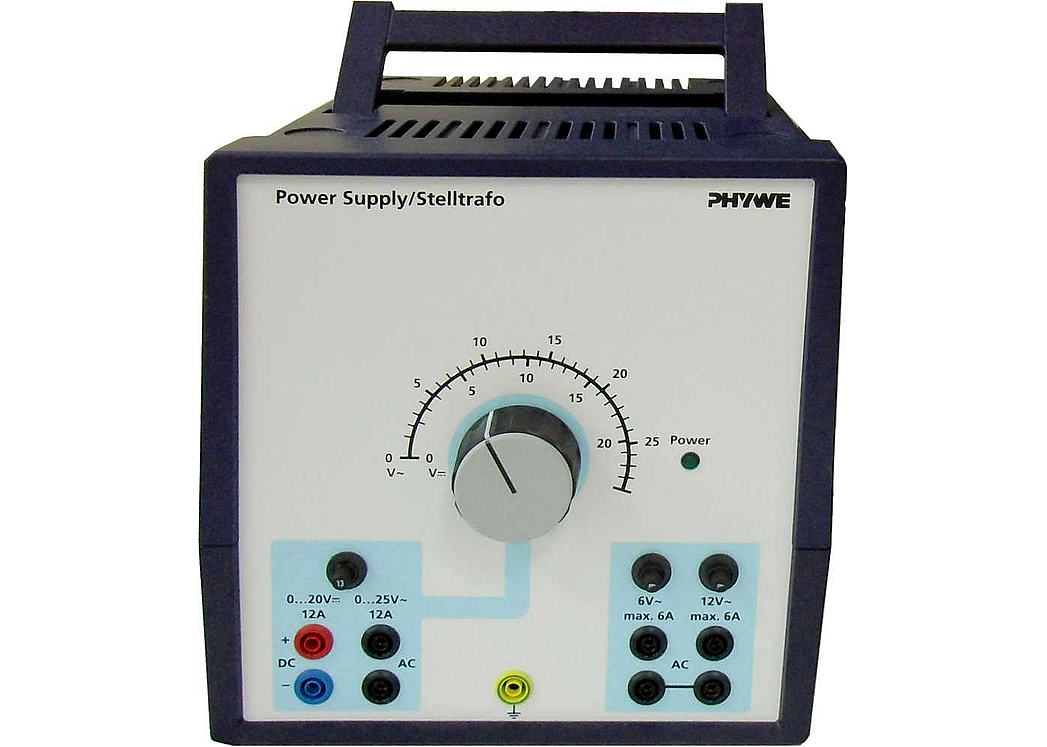
\includegraphics[width=1\linewidth]{Power_supply}
			\caption{Джерело живлення}
			\label{pic:Power_supply}
		\end{tornpage}
	\end{minipage}
	%---------------------------------------------------------
\end{figure}

%=========================================================
\begin{figure}[h!]\centering
	%---------------------------------------------------------
	\begin{minipage}[t]{0.45\linewidth}\centering
		\begin{tikzpicture}[scale=1.5]
			\draw  (0,0) node[contact] {} -- ++(0,1) to[ampermeter] ++(4,0) -- ++(0,-1) -- ++(-0.5,0) node[above right] {$2$};
			\draw  (0,-1) node[contact] {} -- ++(0,-1) -- ++(2.25,0) -- ++(0,1)  -- ++(0.5,0) node[below left] {$2$};
			\fill[red!50, draw=red] (3.3,0.25) rectangle +(0.2,-1.5);
			\fill[red!50, draw=red] (2.75,0.25) rectangle +(0.2,-1.5);
			\draw (2.75,0) node[above left] {$1$} -- ++(-0.5,0)  -- ++(0,0.5) -- ++(0.85,0) -- ++(0,-2) -- ++(0.9,0)  -- ++(0,0.5)  -- ++(-0.5,0) node[below right] {$1$};
			\node at (0,-0.5) {$I \le 3$~А};
		\end{tikzpicture}
		\caption{Схема з'єднання котушок}
		\label{pic:scheme_for_Helmholtz}
	\end{minipage}
	%---------------------------------------------------------
	\begin{minipage}[t]{0.45\linewidth}\centering
		\begin{tikzpicture}[scale=1.5]
			\draw  (0,0) node[contact] {} -- ++(0,0.9) to[ampermeter] ++(2,0) -- ++(0,-1.25) -- ++(0.5,0) coordinate (A) ;
			\draw  (0,-1) node[contact] {} -- ++(0,-0.9) to [resistor={adjustable}] ++(2,0) -- ++(0,1.25) -- ++(0.5,0) coordinate (B) ;
			\draw[ultra thick, red!30] ([shift={(0.47,-0.22)}]A) circle (0.5);
			\draw[ultra thick, red!30] ([shift={(0.47,-0.27)}]A) circle (0.5);
			\draw[ultra thick, red!50] (A) node[contact] {} ++(180:0) arc (160:-165:0.5) node[contact] {};
			\node at (0,-0.5) {$I \le 2$~A};
		\end{tikzpicture}
		\caption{Схема з'єднання контура}
		\label{pic:scheme_for_coil}
	\end{minipage}
	%---------------------------------------------------------
\end{figure}
%=========================================================

\begin{More}
	Нульова точка відліку крутильних терезів має часто перевірятися, оскільки швидкий обертальний рух пристроя, а також кожне стороннє втручання (заміна контуру, заміна кута, тощо) може зашкодити її положенню.
\end{More}

\section{Хід роботи}

\begin{enumerate}
	\item Збираємо лабораторну установку (рис.~\ref{pic:Experimental_installation}). Одне джерело струму (рис.~\ref{pic:Power_supply}) через амперметр приєднується до котушок Гельмгольца (рис.~\ref{pic:scheme_for_Helmholtz}), інше --- до контуру (рис.~\ref{pic:scheme_for_coil}). Треба простежити, щоб провідники, які підводять струм до контуру не спричиняли додатковий обертальний момент. Крутильні терези мають бути встановлені таким чином, щоб контур знаходився точно в центрі між котушками.
	\item \textbf{Дослід 1.} \emph{Зніміть залежність обертального моменту $M$ від сили струму в контурі $I'$.} Для цього використовуйте найбільший за діаметром контур з найбільшим числом витків $N$. Встановіть найбільший струм $I = 3$~А через котушки Гельмгольца і кут $\alpha = 90^\circ$.
	\item \textbf{Дослід 2.}  \emph{Зніміть залежність обертального моменту $M$ від сили струму в через котушки Гельмгольца $I$.} Для цього використовуйте найбільший за діаметром контур з найбільшим числом витків $N$. Встановіть найбільший струм $I' = 2$~А через контур і кут $\alpha = 90^\circ$.
	\item \textbf{Дослід 3.} \emph{Зніміть залежність обертального моменту $M$ від кута $\alpha$} в інтервалі $-90\ldots 90^\circ$ з кроком $15^\circ$.  Для цього використовуйте найбільший за діаметром контур з найбільшим числом витків $N$. Встановіть найбільший струм $I' = 2$~А через контур і котушки Гельмгольца $I = 3$~А. Кут $\alpha$ слід змінювати використовуючи позначки на пристрої, що тримає котушку. Позначки на нерухомій частині пристрою зроблено через $45^\circ$, а на рухомій --- через $30^\circ$. Таким чином, суміщаючи відповідні позначки, можна забезпечити крок в  $15^\circ$.
	\item \textbf{Дослід 4.} \emph{Зніміть залежність обертального моменту $M$ від квадрату діаметру петлі $d^2$}. Для цього використовуйте найбільший за діаметром контур з найбільшим числом витків $N$. Встановіть найбільший струм $I' = 2$~А через контур і котушки Гельмгольца $I = 3$~А та кут $\alpha = 90^\circ$.
	\item \textbf{Дослід 5.} \emph{Зніміть залежність обертального моменту $M$ від кількості витків $N$}.  Встановіть найбільший струм $I' = 2$~А через контур і котушки Гельмгольца $I = 3$~А та кут $\alpha = 90^\circ$.
\end{enumerate}

\section{Завдання}
\begin{enumerate}
	\item За результатами дослідів $1 - 5$ побудуйте графіки залежності обертального моменту від усіх досліджуваних параметрів:
	      \begin{itemize}
		      \item Для досліду 1 --- $M = M(I')$;
		      \item Для досліду 2 --- $M = M(I)$;
		      \item Для досліду 3 --- $M = M(\sin\alpha)$;
		      \item Для досліду 4 --- $M = M(d^2)$;
		      \item Для досліду 5 --- $M = M(N)$;
	      \end{itemize}
	\item З лінійної апроксимації відповідних залежностей для кожного досліду, визначте константу котушок Гельмгольца, використовуючи формулу~\eqref{eq:TorqueE}.
	\item Порівняйте отримані значення з таким, що розрахований за законом Біо-Савара-Лапласа~\eqref{val:Helmhottz_constant}.
\end{enumerate}

\section*{Контрольні запитання}

\begin{enumerate}
	\item Що таке магнітна індукція та одиниці її вимірювання в SI та СГС? Як визначається напрямок вектора $\vec{B}$? Що таке лінії магнітної індукції?
	\item Що таке вектор $\vec{H}$ та одиниці його вимірювання в SI та СГС?
	\item Що таке магнітний диполь? Чим він характеризується? Наведіть прик\-лади.
	\item Як розрахувати магнітний момент контура зі струмом?
	\item Як визначається магнітне поле магнітного диполя.
	\item У чому полягає закон Біо-Савара-Лапласа? Яка магнітна індукція поля, створюваного елементом струму?
	\item Як виглядають лінії магнітної індукції поля витка зі струмом?
	\item Які сили діють на контур зі струмом в однорідному магнітному полі? Як розрахувати величину крутного моменту цих сил?
\end{enumerate}

\section*{Розрахункові завдання}

\begin{enumerate}
	\item Розрахуйте магнітну індукцію поля на осі кругового витка зі струмом в його центрі і на відстані $r$ від центру?
	\item З закону Біо-Савара-Лапласа виведіть значення константи котушок Гельмгольца.
	\item Розрахуйте магнітне поле нескінченно довгого провідника зі струмом $I$ на відстані $r$. Як розрахувати магнітне поле частини такого провідника? Наведіть розрахунки.
	\item Розрахуйте магнітний момент однорідно зарядженої кулі радіусом $R$, що обертається із кутовою швидкістю $\omega$. Заряд кулі $Q$. Як знайти магнітний момент, якщо замість кулі буде циліндр радіусом $R$?
\end{enumerate}

\end{document}
